\chapter{Specifiche Wi-Fi Direct}
\label{chap:basi}

\begin{minipage}{12cm}\textit{
Wi-Fi Direct, nominato anche Wi-Fi P2P, è una tecnologia
che consente la comunicazione da dispositivo a dispositivo in Wireless
LAN.
Consente ai dispositivi abilitati Wi-Fi Direct di negoziare e selezionare
dinamicamente
uno dei dispositivi mobili come Group Owner. Group Owner del gruppo
svolge
il ruolo di Access Point come nella modalità dell'infrastruttura Wi-Fi
classica. Il protocollo
Wi-Fi Direct è stato inizialmente rilasciato per connettere al volo dispositivi
abilitati Wi-Fi.
Tuttavia, grazie alle funzionalità avanzate, il protocollo può essere
utilizzato in diverse
applicazioni come trasferimento di file, condivisione di risorse, giochi
online, diffusione di
allerta, social networking, ecc.}

\end{minipage}

\vspace*{1cm}

\section{Panoramica tecnica}

\begin{figure}
\caption{rete Wi-Fi Direct}
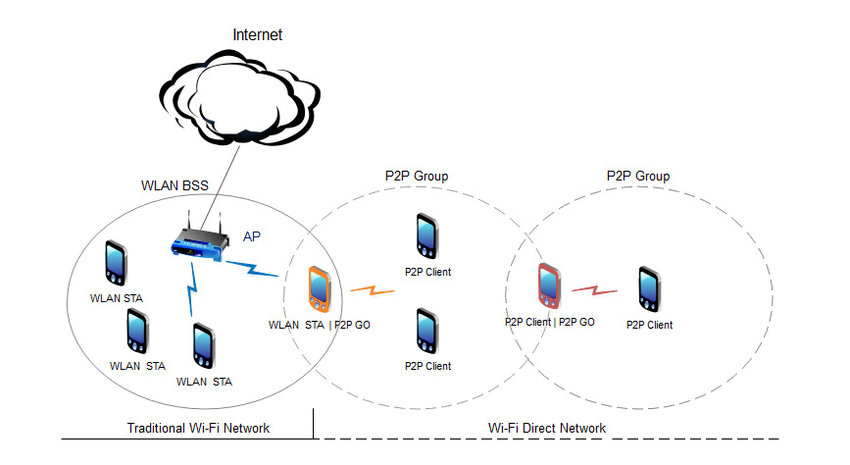
\includegraphics[width=1\columnwidth]{imgs/wifip2pnet.jpg} % Example image
\end{figure}


\label{sec:sezioni}
Wi-Fi Alliance ha introdotto nel 2010 la tecnologia Wi-Fi Direct per consentire
ai dispositivi
Wi-Fi di connettersi direttamente tra loro senza connettersi a un Access Point
(AP). Wi-Fi Direct,
inizialmente chiamato WiFi Peer-to-Peer (Wi-Fi P2P), è basato sulla modalità
dell'infrastruttura
IEEE 802.11 e offre una comunicazione dispositivo-dispositivo diretta, sicura e
rapida. Il recente
Wi-Fi P2P Technical Specification \cite{alliance2016wi} è stato rilasciato nel
2016 (versione 1.7).
I dispositivi abilitati Wi-Fi Direct si scoprono e formano un gruppo P2P. In
ciascun gruppo P2P,
un nodo eletto, chiamato Group Owner (GO) P2P, funge da AP.


Wi-Fi Direct consente a dispositivi Wi-Fi come smartphone, laptop, smart TV,
stampanti, fotocamere e altri dispositivi di connettersi in modo rapido e
comodo senza
l'aggiunta di un Access Point (AP). Wi-Fi Direct è basato sulla
l'infrastruttura
della WLAN. Le connessioni Wi-Fi Direct sono protette
con Wireless Protected Access - 2 (WPA2) \cite{mathews2007evolution}.
Wi-Fi Direct supporta le stesse elevate velocità di trasmissione dati del Wi-Fi
(fino a 250 Mbps).
La portata della connessione Wi-Fi Direct è di 200 metri (questa è la portata
teorica e la portata
pratica potrebbe essere minore). Le specifiche richiedono inoltre una
connessione
1: 1 obbligatoria per i dispositivi certificati Wi-Fi Direct, in cui mantenere
la funzione
opzionale 1: N. Nelle sezioni successive,
forniamo una panoramica dettagliata delle funzionalità Wi-Fi Direct.



\section{Architettura di rete}



L'entità funzionale dell'architettura Wi-Fi Direct è denominata
"Gruppo P2P" che è funzionalmente equivalente a un Basic Service Set
(BSS) nella rete Wi-Fi legacy. Un gruppo P2P è costituito da un proprietario
di un gruppo P2P (P2P GO) e zero o più client P2P. Il P2P GO
è anche chiamato Soft-AP. Le funzioni AP sono implementate nei dispositivi P2P
Wi-Fi.
Un dispositivo P2P può assumere dinamicamente il ruolo di un AP o di un client.
I ruoli
dei dispositivi P2P (ad esempio P2P GO e P2P Client) vengono solitamente
negoziati prima
di creare un gruppo P2P e rimangono fissi mentre il gruppo P2P è attivo. La
Figura 2.1 illustra
i diversi ruoli dei dispositivi P2P.



\section{Device Discovery}




Device Discovery è una funzione obbligatoria che deve essere supportata
da tutti i dispositivi P2P. Prima di formare un gruppo P2P, un dispositivo
P2P esegue la procedura Rilevamento dispositivo per rilevare la presenza di
altri dispositivi P2P nel suo intervallo wireless. La procedura consiste in
due fasi distinte: Scansione e Trova. Nella fase di scansione, il dispositivo
P2P esegue la tradizionale scansione Wi-Fi (scansione passiva) attraverso
tutti i canali supportati al fine di raccogliere informazioni sui dispositivi
circostanti, i gruppi P2P e le reti Wi-Fi legacy. Una volta completata la
fase di scansione, il dispositivo entra nella fase di ricerca. Nella
fase di ricerca, il dispositivo P2P si alterna tra due stati: Cerca
e Ascolta. Nello stato Cerca, il dispositivo P2P invia uno o più
frame Probe Request (PREQ)

sul canale social, ovvero i canali 1, 6 e 11 nella banda dei 2,4 GHz.
Nello stato di ascolto, il dispositivo P2P si sofferma su uno dei canali
social (1, 6 e 11) chiamato canale Listen e attende i frame Probe Request
(PREQ) da altri dispositivi P2P. Quindi, il successo della fase di ricerca
è quello in cui due dispositivi arrivano a un canale comune per comunicare.
È evidente che il processo di Rilevamento dispositivo P2P può indurre
qualche ritardo a un dispositivo P2P per scoprire tutti i
dispositivi P2P nella sua posizione iniziale. Questo ritardo, definito
"Ritardo rilevamento dispositivo", può essere relativamente elevato se
diversi dispositivi P2P eseguono contemporaneamente Rilevamento dispositivo
nello stesso intervallo wireless. La figura 2.2 illustra la procedura di
rilevamento dei dispositivi P2P in Wi-Fi Direct.

\begin{figure}
\caption{Fase di discovery}
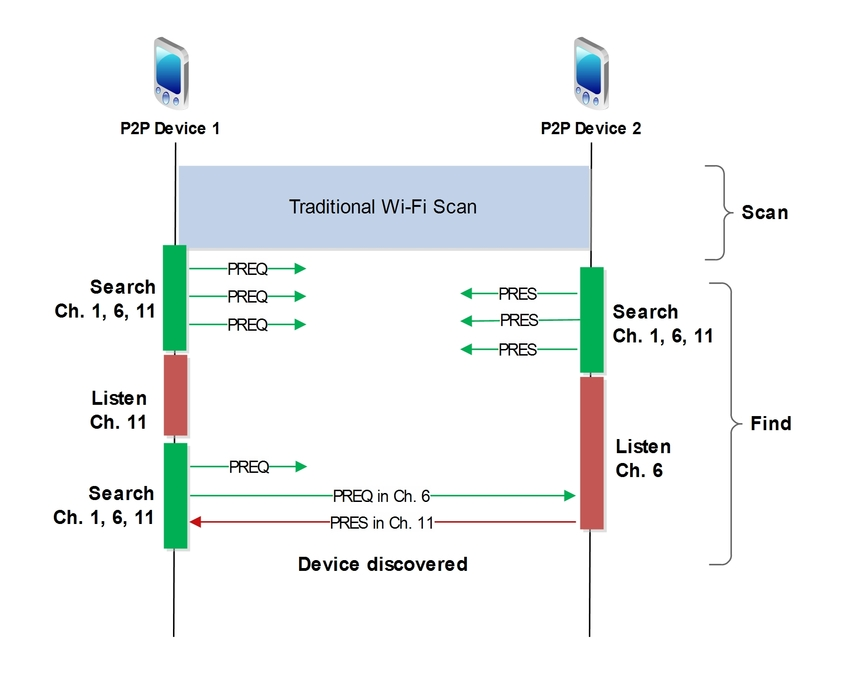
\includegraphics[width=1\columnwidth]{imgs/DeviceDiscovery.jpg} % Example image
\end{figure}


\section{Service Discovery}
Service Discovery è una
procedura opzionale in Wi-Fi Direct. La procedura inizia dopo il
rilevamento dei dispositivi e prima della procedura di formazione dei
gruppi. Consente a un dispositivo P2P di connettersi ad altri dispositivi
P2P solo se quest'ultimo fornisce il servizio previsto. Utilizzando la
procedura di individuazione del servizio, un dispositivo P2P pubblicizza
i servizi disponibili utilizzando il protocollo GAS
(Generic Advertisement Service) \cite{wikipedia_2015}.
Wi-Fi Alliance ha definito una serie di servizi standard supportati
da Wi-Fi Direct come Play, Send e Print \cite{wi-fialliance}





\section{Formazione Gruppi}

In seguito al successo di Device Discovery (procedura obbligatoria) e
Service Discovery (procedura facoltativa), i dispositivi P2P  possono
stabilire il gruppo P2P. Durante la Formazione di gruppo, il dispositivo
sarà GO sarà determinato . Come descritto in Figura 2.3 ci sono
tre schemi di formazione dei gruppi P2P possibili in

Wi-Fi Direct: (1) Formazione di gruppo standard (2) Formazione di
gruppi autonomi e (3) Formazione di gruppi permanenti. Nella formazione
di gruppi standard, presentata nella figura 2.3,  due dispositivi P2P
negozieranno
tra loro il chi sarà GO . La negoziazione del GO è un handshake a
tre vie. Durante l'handshake, i due dispositivi inviano tra loro un valore
numerico scelto a caso chiamato "Intent value". L'Intent value
va da 0 a 15 e misura il desiderio del dispositivo P2P di essere il P2P
GO. Il dispositivo P2P che invia il valore di Intento più elevato
diventa GO.Nel caso in cui entrambi i dispositivi inviano
lo stesso Intent value, viene utilizzato
un bit di breaker per la decisione e il dispositivo con il bit breaker  
impostato a uno diventa il GO.

\begin{figure}
\caption{tipi di gruppi Wi-Fi Direct}
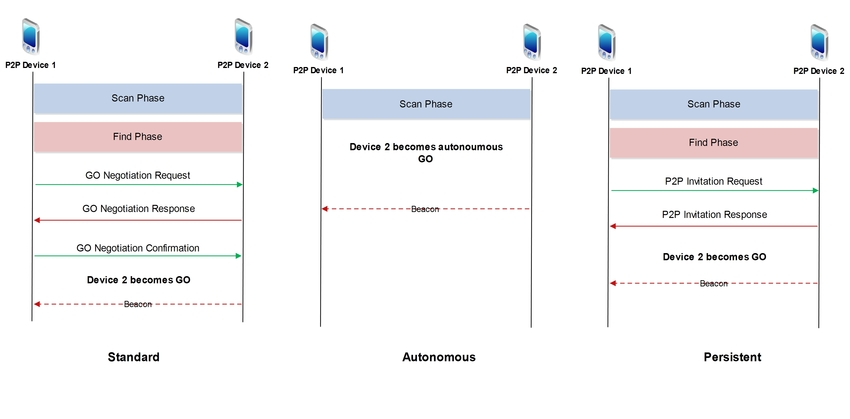
\includegraphics[width=1\columnwidth]{imgs/wifiGroup.jpg} % Example image
\end{figure}


La Figura 2.4 mostra il confronto del valore
dell'Intent tra due dispositivi P2P durante la Formazione di gruppi
standard. Il dispositivo P2P selezionato come P2P GO avvierà una
sessione di gruppo P2P. L'altro dispositivo P2P può quindi
connettersi al P2P GO per ottenere credenziali e scambiare
dati. Allo stesso modo, altri dispositivi P2P e dispositivi
Wi-Fi legacy possono unirsi al gruppo P2P come client. Nella
formazione di gruppi autonomi, illustrata nella figura 2.3,
il ruolo di GO non è negoziato. Un dispositivo P2P
si annuncia come GO e inizia a inviare i beacon. Questo
processo è molto simile al Wi-Fi legacy in cui un AP
invia direttamente Beacons nella rete per diventare
rilevabile. La formazione di gruppi autonomi è più
semplice e più veloce della formazione di gruppi
standard. nella formazione di gruppi persistenti, come illustrato
nella figura 2.3, un dispositivo P2P invia un invito
a un altro dispositivo P2P, precedentemente collegato
ad esso in un gruppo P2P, per ristabilire il gruppo P2P.
Questo si ottiene usando i frame Invitation Request e P2P
Invitation Response di P2P. Il ruolo di ciascun dispositivo
P2P deve rimanere uguale a quello del gruppo P2P precedentemente
formato.
\begin{figure}
\centering
\caption{comparazione Intent Value}
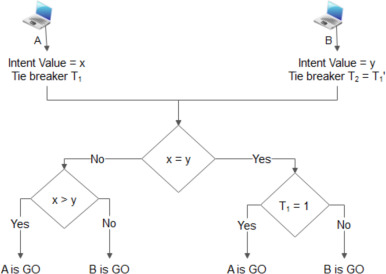
\includegraphics[width=0.9\columnwidth]{imgs/intentValueComparison.jpg} %
%Example image

\end{figure}
Per stabilire un gruppo persistente, i dispositivi P2P
devono dichiarare il gruppo P2P come persistente durante la formazione
standard o autonoma del gruppo.
dei flag bit all'interno dei beacon P2P,dei telegrammi Probe
Response e nella GO Negotiation vengono utilizzati
per indicare che il gruppo P2P è persistente o no.
Se il flag bit non è impostato durante la procedura di formazione dei
gruppi, i dispositivi P2P non possono riattivare un gruppo persistente
in futuro e devono avviare un gruppo standard o autonomo. La specifica
Wi-Fi Direct \cite{alliance2016wi} definisce le procedure di formazione di
gruppi standard
e permanenti solo tra due dispositivi P2P. Gli altri dispositivi P2P i ricerca
possono essere aggiunti, a gruppi P2P formati in precedenza.



\section{Sicurezza}

Wi-Fi Direct richiede a tutti i dispositivi P2P di
implementare Wi-Fi Protected Setup (WPS) \cite{WPS} al fine di
proteggere il processo di creazione della connessione e della
la comunicazione nel Gruppo P2P. Nello schema WPS, il
P2P GO implementa il Registrar interno in cui il client
P2P implementa Enrollee. Lo schema WPS funziona in due fasi.
Nella fase 1, il Registrar interno genera e invia le credenziali
di rete per iscriversi. Nella fase 2, l'iscritto (Client P2P)
si ricollega al Registrar interno (P2P GO) utilizzando le
nuove credenziali



\section{Risparmio energetico}

Il Wi-Fi legacy utilizza il risparmio energetico utilizzando le modalità
Sleep e Active per gli STA Wi-Fi (client). La maggior parte degli AP
tradizionali sono permanentemente collegati a una normale fonte di
alimentazione e, quindi, non hanno bisogno di alcuna funzione di risparmio
energetico. Tuttavia, in Wi-Fi Direct, il P2P GO, che funge da Soft-AP,
può essere un dispositivo alimentato a batteria e ha una durata limitata.
Quindi,
Wi-Fi Direct introduce due nuovi schemi per il risparmio energetico nei
dispositivi P2P. Questi schemi sono: (1) Opportunistic Power Save
(OppPS) e (2) Notice of Absence (NoA). Nello schema OppPS, il GO è
autorizzato a risparmiare energia quando i suoi clienti sono in
modalità Sleep. Il GO annuncia il suo periodo di presenza chiamato
"CTWindow". Alla fine della CTWindow, se tutti i nodi sono in modalità
Sleep, il GO può anche andare in modalità Sleep fino al prossimo Beacon.
Tuttavia, alla fine della CTWindow, se uno dei nodi Client P2P è in
modalità attiva, il GO deve rimanere attivo fino al prossimo beacon.
Nello schema NoA, il GO annuncia tramite i frame Beacons e Probe
Response, un "periodo di assenza". Durante il periodo di assenza,
i suoi client non possono accedere al canale, quindi il GO spegne
la sua radio per risparmiare energia utilizzata in trasmissione o
ricezione. Il periodo di assenza viene annunciato in Beacons
utilizzando NoAschedule, costituito da quattro parametri: 1)
Durata - la durata del periodo di assenza, 2) Intervallo - il
tempo tra due periodi di assenza consecutivi, 3) Ora inizio -
l'ora di inizio del primo periodo di assenza dopo l'attuale Beacon
e 4)  Count: il numero di periodi di assenza nel
NoA scheduling corrente. La specifica Wi-Fi Direct non
definisce i valori di questi parametri.




